\documentclass[12pt]{article}
\usepackage[style=numeric, sorting=none]{biblatex}
\addbibresource{references.bib}
\usepackage[margin=2.0cm]{geometry}
\usepackage{relsize}
\usepackage{graphicx}
\usepackage{authblk}
\usepackage{hyperref}
\usepackage{caption}
\usepackage{color, colortbl}
\usepackage{float}
\usepackage{amsmath}

\title{\bfseries{Modeling Variability of Intensive Care Unit Demand: a Comparative Cost Analysis and Performance Evaluation of Fixed versus Variable Beds structures with a simulation approach.}}
\date{}

\makeatletter
\renewcommand\AB@affilsepx{, \protect\Affilfont}
\makeatother

\author[1,2,*]{L. Querci}
\author[3]{O. Sagliocco}
\author[4]{B. Er}
\author[5]{F. Mulazzani}
\author[5]{B. Brunoni}
\author[6]{A. Arslantas}
\author[7]{M. K. Arslantas}

\affil[1]{Anesthesia and Intensive Care Residence At University of Bologna, Italy}
\affil[2]{Grande ospedale Metropolitano Niguarda Ca' Grande, Milan, Italy}
\affil[3]{ASST Bergamo Est, Italy}
\affil[4]{University of Health Sciences, Ankara Bilkent City Hospital, Turkey}
\affil[5]{Anesthesia and Intensive Care Residence At University of Milano-Bicocca, Italy}
\affil[6]{Fenerbahçe University, Istanbul, Turkey}
\affil[7]{Demioglu Bilim University, Istanbul, Turkey}
\affil[*]{Corresponde author. Email querci.lorenzo@gmail.com}

\definecolor{Gray}{gray}{0.9}

\begin{document}

%TC:ignore
\pagenumbering{gobble}
\maketitle
\begin{center}
{\LARGE
\underline{Abstract}
}
\end{center}
%TC:endignore

{\large\noindent\normalsize

\noindent\textbf{Introduction. }High demand, limited intensive care unit (ICU) beds, and costs pose a sustainability challenge in healthcare. Simulation modelling helps examine ICU bed assignment
policies.\cite{kusum_2015} Our study compares the performance of two management strategies: fixed
versus variable bed availability. Estimating length of stay (LOS) is a complex process \cite{bahalkeh_relationship_2022, verburg_et_al_which_2017} due to ICU daily uncertainties: we developed an ICU LOS prediction model integrated into a complex simulation model.\\

\noindent\textbf{Materials and Method. }Anonymized data of adult patients from \textit{AmsterdamUMCdb} (2003-2016) were used. Admission rate (AR) was estimated from elective and urgent patients cumulative AR. Using coefficients for four-time slots and days of the week, we estimated the lambda parameter of a Poisson distribution and simulated random admissions. The best fixed-bed ICU was which one minimises costs: a Monte Carlo (MC) simulation was performed on a bed occupancy algorithm (Image \ref{fig:algSim}), a stochastic bootstrapping LOS simulation\cite{bai_managing_2021}. ICU
bed cost was 1425 Euros/day, with fixed costs 0.43.\cite{lefrant_daily_2015}  In a closed system, a patient unsuccessfully demanding ICU was considered rejected. According to literature, each
urgent life saved costs 111,035 Euros \cite{edbrooke_implications_2011} delayed elective procedures costs 1,000 Euros, resulting in 21,927.22 Euros per rejected patient. MC simulation produces the
outcomes: \(\ Rejection Index = \frac{{\text{Patients Rejected}}}{{\text{Days Simulation}}}\) and \(\ Free Free Beds Index = \frac{{\text{Hours Free Beds}}}{{\text{Days Simulation}}}\). The optimal number of beds has been determined by minimising the product of these values and their associated expenses. LOS prediction was obtained from a regression random forest model and a stochastic approach. MAE, MSE and RMSE confronted different models in a subset test. A complex model that incorporates optimal variation in the number of beds within a range of 0.875 to 1.125 times the calculated ideal bed capacity was built. A probability score executed every 24 hours allowed for the opening or closing of variable beds seven days in advance. The prediction model was based on an MC simulation that considered the estimation of remaining LOS for admitted patients, the estimation of incoming patients for the next seven days, and a stochastic estimation of LOS for these patients. Another MC simulation was used to optimize this probability cut-off to minimise costs. The results in terms of costs of fixed and variable bed simulations were compared using an MC simulation.\\

\noindent\textbf{Results. }The admission ratio was 0.19 patients/hour. Elective-to-urgent admission ratio was 2.70. The best number which minimises ICU beds in the fixed model was n=42 (Image \ref{fig:fixBedNumberCostMinimization}) which resulted in a cost of €1865.276±€2488.486 for rejected patients and €7,412.416±€1,592.51 for unused beds (total daily cost of €9,277.692±€2,954.429). The
random forest regression model showed a bad test accuracy (0.40) without overfitting. After probability coefficient optimisation, Variable-Beds ICU resulted in a total daily cost of €10,728.200±€4,296.201.\\

\noindent\textbf{Conclusion. }In a healthcare system that daily faces the presence of limited resources, a variable-bed intensive care model that meets patient needs while allowing for well-planned resource allocation can offer advantages.}\\

%TC:ignore

\begin{figure}[H]
\centering
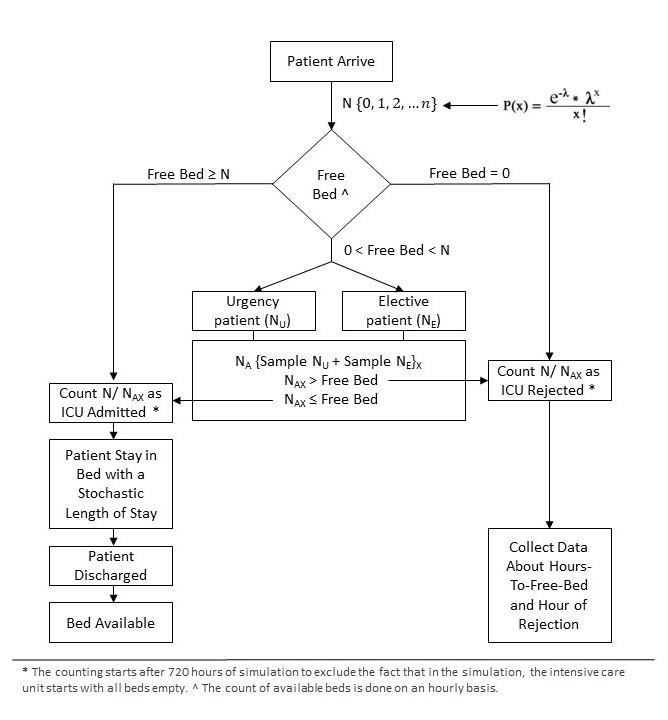
\includegraphics[width=0.8\textwidth]{Image1.jpeg}
\caption{The algorithm considers an admission rate based on an hourly probability distribution following a Poisson distribution with lambda derived from the array of admission coefficients \ref{tab:electiveCoefAdmRate} \ref{tab:urgencyCoefAdmRate}. The length of stay (LOS) is modeled stochastically by bootstrapping from the LOS distribution in the database. This type of simulation allows for the extraction of two parameters considered for cost analysis: the number of patients rejected from the intensive care unit and the number of hours that each intensive care bed remains unused. Firs 30 simulation days were not considered in the result considering that ICU started with all beds empty.}
\label{fig:algSim}
\end{figure}

\begin{figure}[H]
\centering
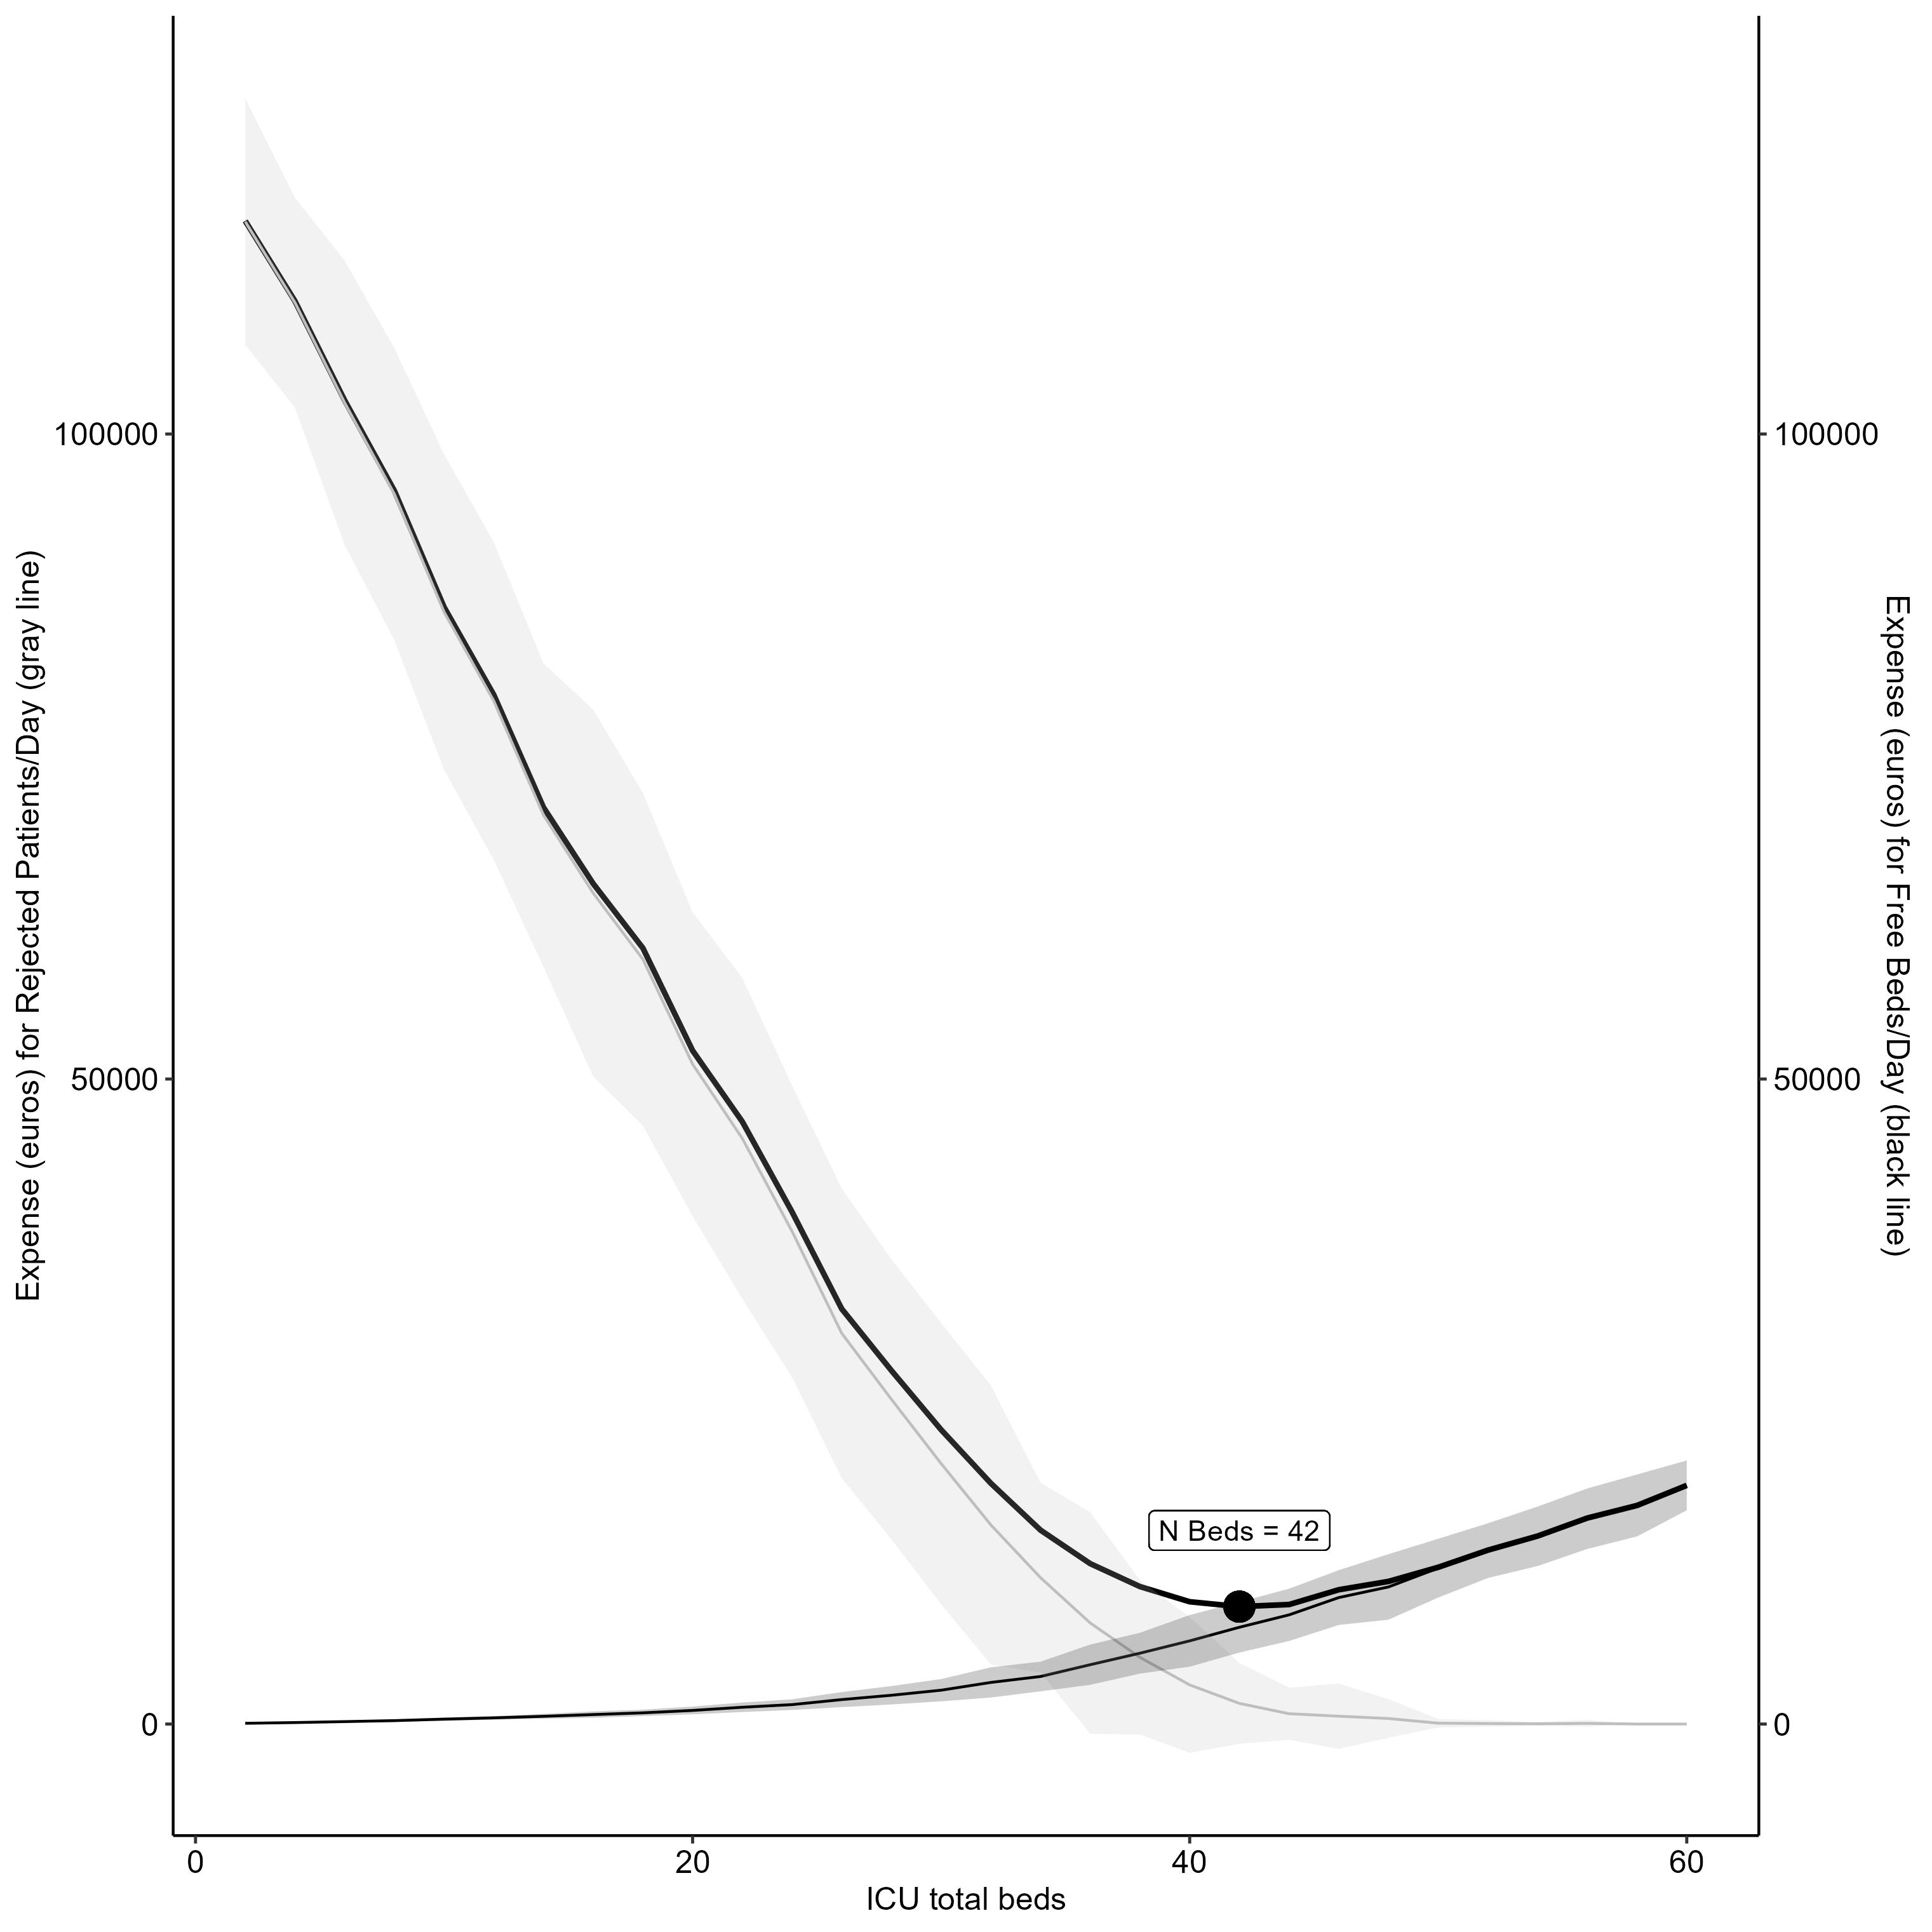
\includegraphics[width=0.8\textwidth]{Image2.jpeg}
\caption{Simulation to find the best number of beds minimizing costs for rejected patients and unused beds.The simulation considers a number of beds ranging from 2 to 60, a simulation duration of 60 days (1440 hours), and a total number of simulations set to S = 100. Cost were based on cost table \ref{tab:costAnalSimulation} in appendix. N = 42 beds minimize cost. Raw data are available in appendix table \ref{tab:bestFixBedSimulationCost}} and \ref{tab:bestFixBedSimulation}.
\label{fig:fixBedNumberCostMinimization}
\end{figure}

\printbibliography

\newpage

\begin{center}
{\LARGE
\underline{Appendix}
}
\end{center}

Files used for the simulation are available with public access in the \href{https://github.com/querci-lorenzo/datathonESICM2023-team3}{GitHub repository}.\\


\begin{table}[H]
\captionsetup{skip=10pt}
\caption{Coefficient for Elective Admission Rate}
\label{tab:electiveCoefAdmRate}
\centering
\begin{tabular}{rrrrrrr}
\hline
1 & 2 & 3 & 4 & 5 & 6 & 7 \\ 
\hline
0.12 & 0.12 & 0.12 & 0.12 & 0.12 & 0.01 & 0.01 \\
0.57 & 0.57 & 0.57 & 0.57 & 0.57 & 0.04 & 0.04 \\
0.24 & 0.24 & 0.24 & 0.24 & 0.24 & 0.02 & 0.02 \\
0.02 & 0.02 & 0.02 & 0.02 & 0.02 & 0.00 & 0.00 \\
   \hline
\end{tabular}
\end{table}

\begin{table}[H]
\captionsetup{skip=10pt}
\caption{Coefficient for Urgency Admission Rate}
\label{tab:urgencyCoefAdmRate}
\centering
\begin{tabular}{rrrrrrr}
\hline
1 & 2 & 3 & 4 & 5 & 6 & 7 \\
\hline
0.06 & 0.06 & 0.06 & 0.06 & 0.06 & 0.06 & 0.06 \\
0.06 & 0.06 & 0.06 & 0.06 & 0.06 & 0.06 & 0.06 \\
0.07 & 0.07 & 0.07 & 0.07 & 0.07 & 0.07 & 0.07 \\
0.06 & 0.06 & 0.06 & 0.06 & 0.06 & 0.06 & 0.06 \\
   \hline
\end{tabular}
\end{table}

\begin{table}[H]
\captionsetup{skip=10pt}
\centering
\caption{Simulation to find the best number of beds minimizing costs for rejected patients and unused beds: the frequency. The simulation considers a number of beds ranging from 2 to 60, a simulation duration of 60 days (1440 hours), and a total number of simulations set to S = 100. Cost were based on cost table\ref{tab:costAnalSimulation}}
\label{tab:bestFixBedSimulation}
\begin{tabular}{ccc}
\hline
Bed Number & Rejected patients/Bed/Day & Hour available Bed/Day \\
\hline
2 & 5.3113 $\pm$ 0.3400 & 2.247 $\pm$ 0.9178 \\
4 & 5.0252 $\pm$ 0.2901 & 4.4963 $\pm$ 1.5558 \\
6 & 4.6708 $\pm$ 0.3925 & 7.3942 $\pm$ 2.228 \\
8 & 4.348 $\pm$ 0.4036 & 10.3475 $\pm$ 3.1471 \\
10 & 3.9313 $\pm$ 0.4358 & 14.856 $\pm$ 3.9299 \\
12 & 3.6167 $\pm$ 0.4388 & 18.7368 $\pm$ 4.355 \\
14 & 3.2132 $\pm$ 0.4194 & 23.4892 $\pm$ 5.7418 \\
16 & 2.9375 $\pm$ 0.5069 & 28.759 $\pm$ 7.5265 \\
18 & 2.7035 $\pm$ 0.4596 & 34.0033 $\pm$ 7.5753 \\
20 & 2.3327 $\pm$ 0.4198 & 41.3173 $\pm$ 9.186 \\
22 & 2.0702 $\pm$ 0.4432 & 50.9442 $\pm$ 11.3079 \\
24 & 1.742 $\pm$ 0.4031 & 58.9408 $\pm$ 12.6252 \\
26 & 1.3813 $\pm$ 0.4000 & 74.237 $\pm$ 17.8239 \\
28 & 1.1478 $\pm$ 0.3866 & 87.3702 $\pm$ 21.8234 \\ 
30 & 0.9207 $\pm$ 0.3887 & 102.7528 $\pm$ 26.3909 \\
32 & 0.704 $\pm$ 0.3855 & 126.3383 $\pm$ 35.7823 \\
34 & 0.5173 $\pm$ 0.262 & 144.3507 $\pm$ 35.1673 \\
36 & 0.3572 $\pm$ 0.3059 & 180.197 $\pm$ 47.7418 \\
38 & 0.2355 $\pm$ 0.2131 & 215.0863 $\pm$ 48.4461 \\
40 & 0.1383 $\pm$ 0.1877 & 252.5145 $\pm$ 61.2839 \\
42 & 0.073 $\pm$ 0.1116 & 293.7988 $\pm$ 59.9283 \\
44 & 0.0365 $\pm$ 0.072 & 331.49 $\pm$ 62.0244 \\
46 & 0.0277 $\pm$ 0.0902 & 383.9862 $\pm$ 64.9582 \\
48 & 0.0195 $\pm$ 0.0534 & 416.2918 $\pm$ 77.7093 \\
50 & 0.0031 $\pm$ 0.0118 & 473.3305 $\pm$ 69.7185 \\
52 & 0.0018 $\pm$ 0.0088 & 526.467 $\pm$ 64.9048 \\
54 & 0.0009 $\pm$ 0.005 & 570.0527 $\pm$ 70.53 \\
56 & 0.0024 $\pm$ 0.0089 & 623.4448 $\pm$ 71.7614 \\
58 & 0.0000 $\pm$ 0.0000 & 663.6752 $\pm$ 73.4481 \\
60 & 0.0000 $\pm$ 0.0000 & 724.5952 $\pm$ 59.104 \\
\hline
\end{tabular}
\end{table}

\begin{table}[ht]
\captionsetup{skip=10pt}
\centering
\caption{Coefficients of costs related to a patient rejected from the intensive care unit and to an unoccupied bed for 24 hours.}
\label{tab:costAnalSimulation}
\begin{tabular}{rr}
\hline
fixCost (euros) & rejcost (euros) \\
\hline
612.75 & 21,927.22 \\
\hline
\end{tabular}
\end{table}

\begin{table}[H]
\captionsetup{skip=10pt}
\centering
\caption{Simulation to find the best number of beds minimizing costs for rejected patients and unused beds: the expense.The simulation considers a number of beds ranging from 2 to 60, a simulation duration of 60 days (1440 hours), and a total number of simulations set to S = 100. Cost were based on cost table\ref{tab:costAnalSimulation}. N = 42 beds minimize cost.}
\label{tab:bestFixBedSimulationCost}
\begin{tabular}{ccc}
\hline
 Bed Number & Expense for Rejected patients/Day & Expense for Hour available/Day \\
\hline
2 & 116462.79 $\pm$ 7455.07 & 57.37 $\pm$ 23.43 \\
4 & 110187.95 $\pm$ 6361.20 & 114.80 $\pm$ 39.72 \\
6 & 102418.41 $\pm$ 8606.36 & 188.78 $\pm$ 56.88 \\
8 & 95339.57 $\pm$ 8849.79 & 264.18 $\pm$ 80.35 \\
10 & 86203.23 $\pm$ 9556.48 & 379.29 $\pm$ 100.34 \\
12 & 79303.46 $\pm$ 9620.74 & 478.37 $\pm$ 111.19 \\
14 & 70455.82 $\pm$ 9195.92 & 599.71 $\pm$ 146.60 \\
16 & 64411.22 $\pm$ 11114.10 & 734.25 $\pm$ 192.16 \\
18 & 59280.25 $\pm$ 10077.31 & 868.15 $\pm$ 193.41 \\
20 & 51148.90 $\pm$ 9204.22 & 1054.88 $\pm$ 234.53 \\
20 & 45393.01 $\pm$ 9717.19 & 1300.67 $\pm$ 288.70 \\
24 & 38197.22 $\pm$ 8839.45 & 1504.83 $\pm$ 322.34 \\
26 & 30288.81 $\pm$ 8770.16 & 1895.36 $\pm$ 455.07 \\
28 & 25168.80 $\pm$ 8477.38 & 2230.67 $\pm$ 557.18 \\
30 & 20187.66 $\pm$ 8522.05 & 2623.41 $\pm$ 673.79 \\ 
32 & 15436.77 $\pm$ 8452.59 & 3225.58 $\pm$ 913.57 \\
34 & 11343.68 $\pm$ 5745.30 & 3685.45 $\pm$ 897.86 \\
36 & 7831.67 $\pm$ 6706.98 & 4600.65 $\pm$ 1218.91 \\
38 & 5163.86 $\pm$ 4673.36 & 5491.42 $\pm$ 1236.89 \\
40 & 3033.27 $\pm$ 4116.82 & 6447.01 $\pm$ 1564.65 \\
\rowcolor{Gray}
42 & 1600.69 $\pm$ 2447.29 & 7501.05 $\pm$ 1530.04 \\
44 & 800.34 $\pm$ 1579.53 & 8463.35 $\pm$ 1583.56 \\
46 & 607.85 $\pm$ 1978.80 & 9803.65 $\pm$ 1658.46 \\
48 & 427.66 $\pm$ 1170.04 & 10628.45 $\pm$ 1984.02 \\
50 & 67.12 $\pm$ 258.93 & 12084.72 $\pm$ 1780.00 \\
52 & 38.76 $\pm$ 193.69 & 13441.36 $\pm$ 1657.10 \\
54 & 18.65 $\pm$ 109.73 & 14554.16 $\pm$ 1800.72 \\
56 & 52.21 $\pm$ 195.34 & 15917.33 $\pm$ 1832.16 \\
58 & 0.00 $\pm$ 0.00 & 16944.46 $\pm$ 1875.22 \\
60 & 0.00 $\pm$ 0.00 & 18499.82 $\pm$ 1509.00 \\
\hline
\end{tabular}
\end{table}

\begin{figure}[H]
\centering
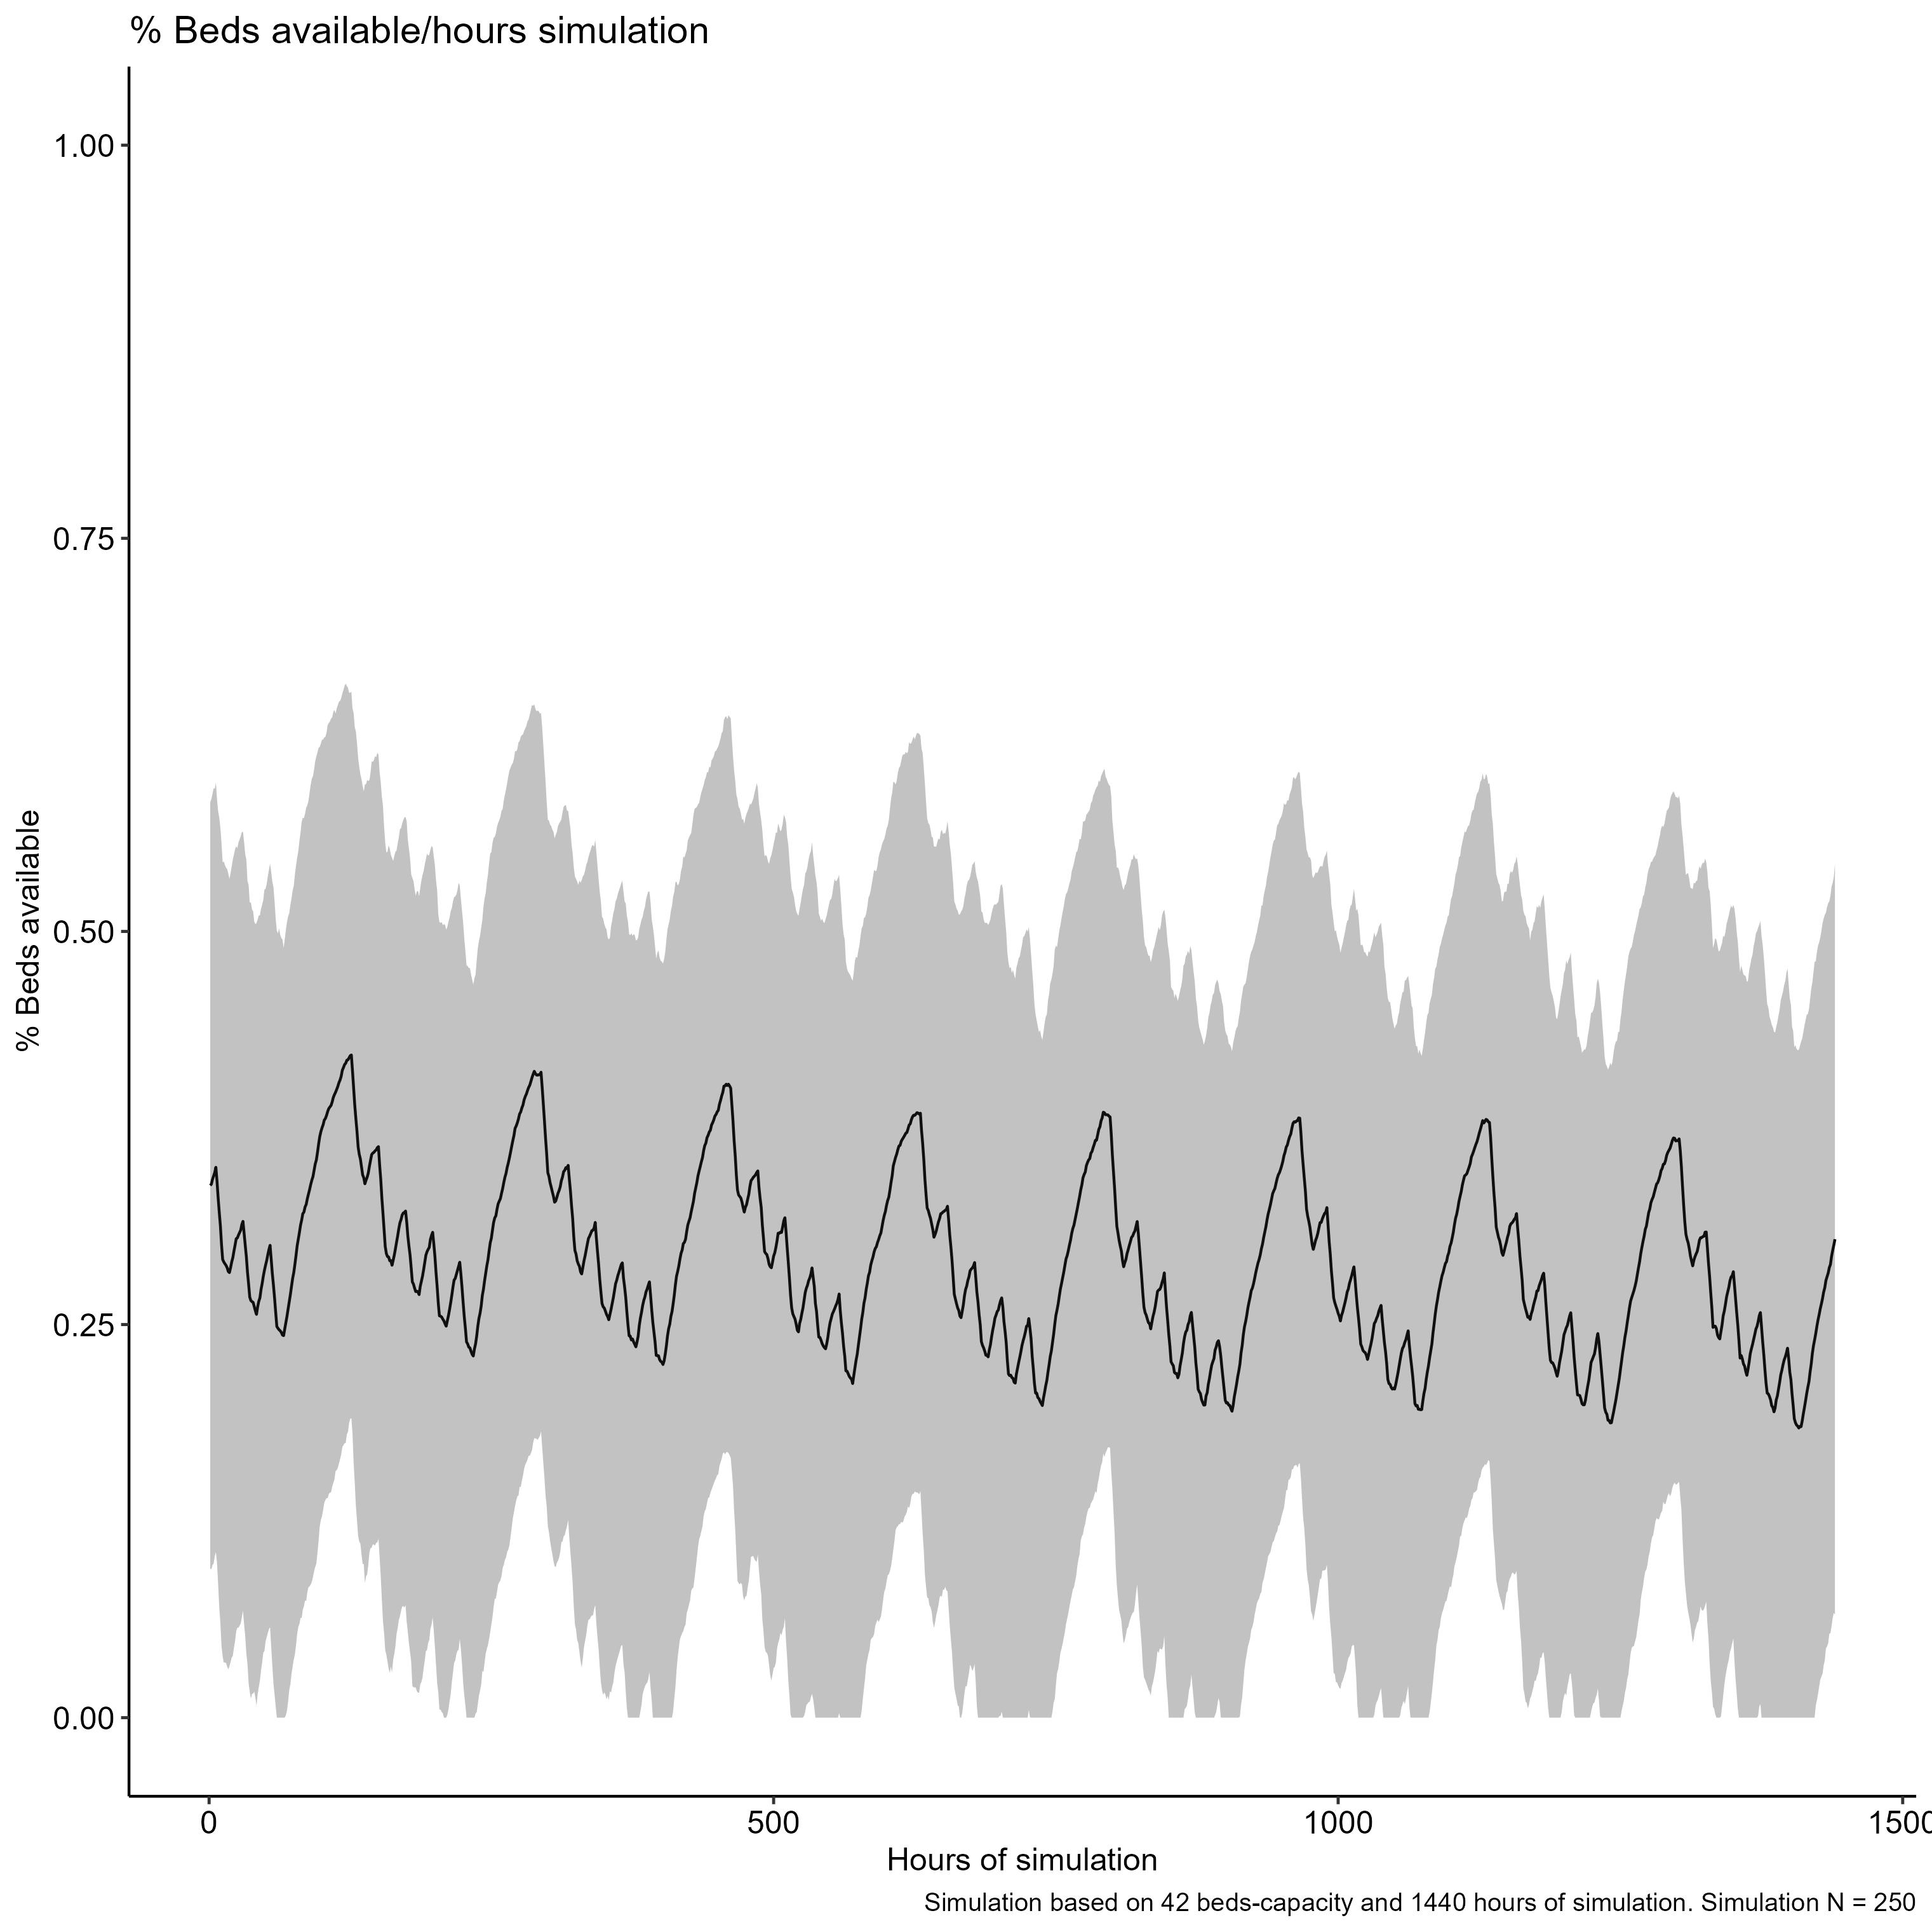
\includegraphics[width=0.8\textwidth]{Image3.jpeg}
\caption{250 simulations of a 42 fixed-bed ICU for sixty days. It is possible to observe changes in bed occupancy for cyclic difference in admission coefficients.}
\label{fig:42bedsSimulation}
\end{figure}

\begin{table}[H]
\captionsetup{skip=10pt}
\centering
\caption{Simulation to find the best coefficient for IntellICU Algorithm to minimize costs. 0.0, which imply simple opening af variable beds result in less cost.}
\label{tab:bestCoefVarBedSimulationCost}
\begin{tabular}{ccc}
\hline
IntellICU Coefficient & Expense for Rejected patients/Day & Expense for Hour available/Day \\
\hline
\rowcolor{Gray}
0.00 & 4531.6262 $\pm$ 3396.3089 & 6050.6594 $\pm$ 1350.5841 \\
0.10 & 4590.0988 $\pm$ 3951.3727 & 6026.4133 $\pm$ 1080.6000 \\
0.20 & 5934.9685 $\pm$ 4063.8637 & 5465.3045 $\pm$ 1082.9104 \\
0.30 & 5934.9685 $\pm$ 4451.7935 & 5345.8182 $\pm$ 1260.7002 \\
0.40 & 7930.3459 $\pm$ 5018.0512 & 5207.4303 $\pm$ 1285.3426 \\ 
0.50 & 6527.0036 $\pm$ 4225.9267 & 5172.0270 $\pm$ 1091.4006 \\
0.60 & 7645.2920 $\pm$ 5410.9119 & 4931.9482 $\pm$ 1300.4846 \\
0.70 & 9180.1977 $\pm$ 6072.5584 & 4724.7110 $\pm$ 1265.2407 \\
0.80 & 8712.4169 $\pm$ 6372.4852 & 4492.4702 $\pm$ 1302.9215 \\
0.90 & 9691.8329 $\pm$ 6066.0916 & 4406.9831 $\pm$ 1116.7737 \\
1.00 & 15926.4735 $\pm$ 7112.5519 & 3211.4057 $\pm$ 777.4318 \\
\hline
\end{tabular}
\end{table}

\begin{figure}[H]
\centering
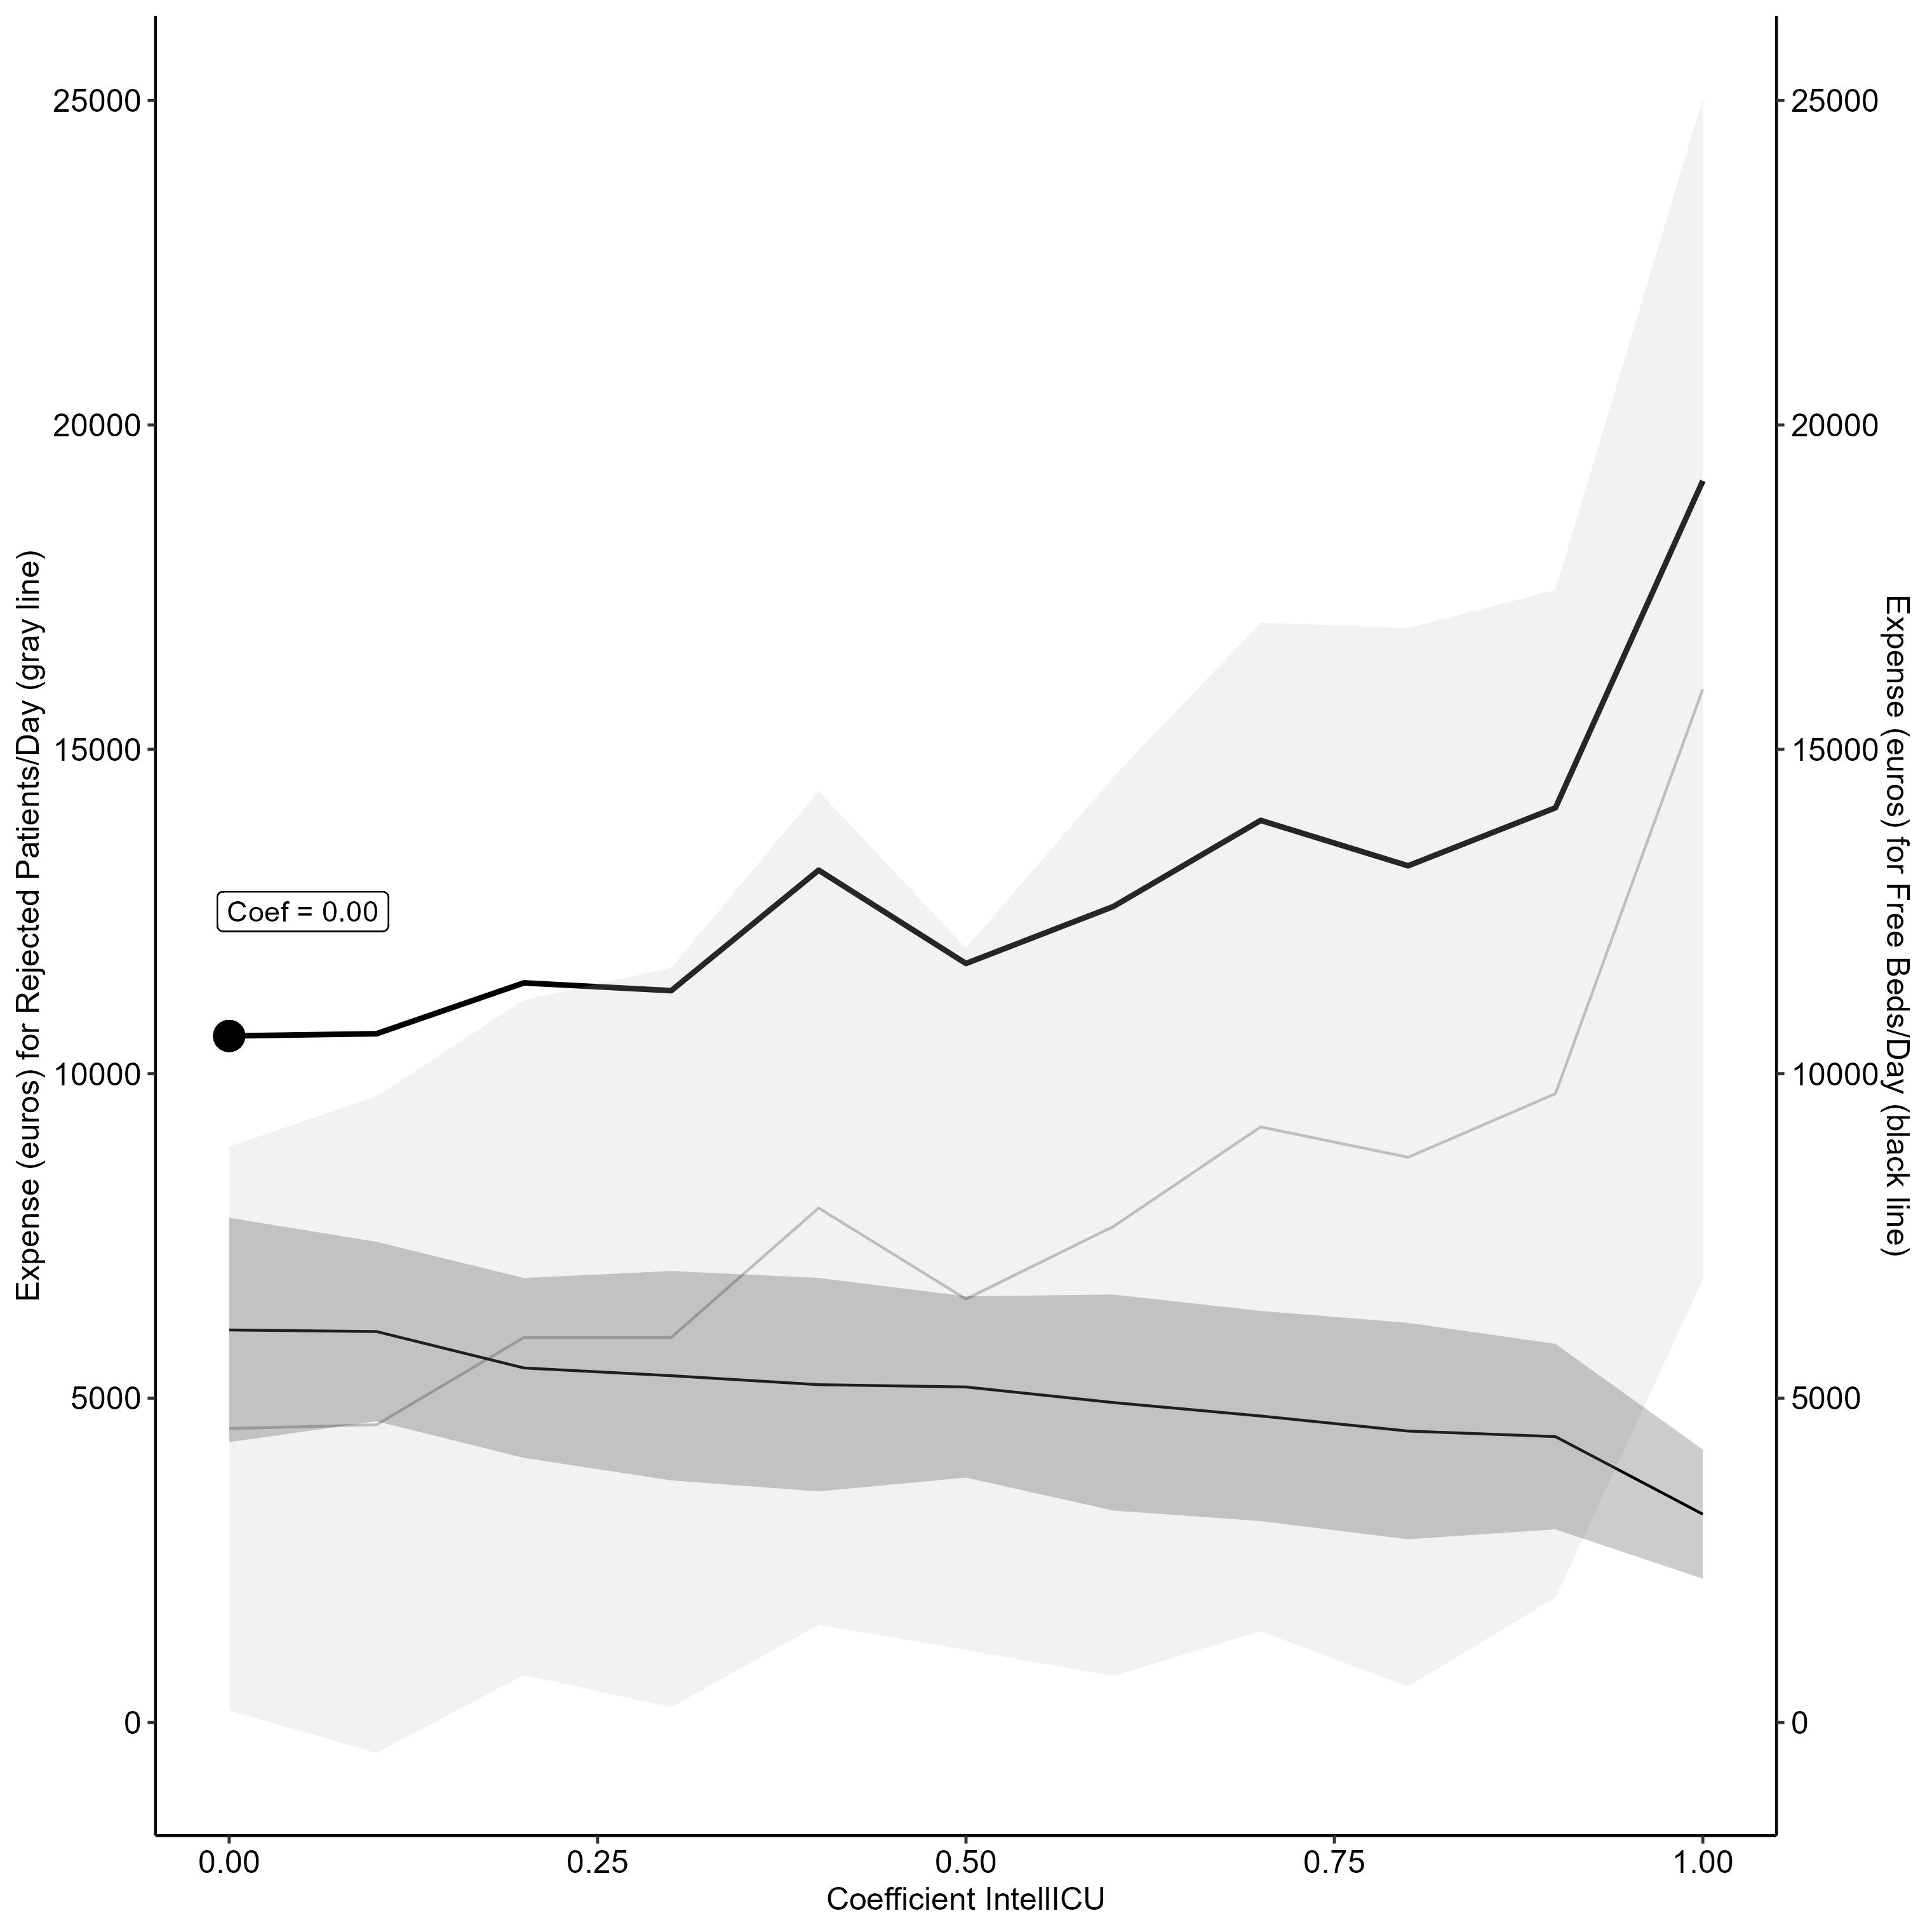
\includegraphics[width=0.8\textwidth]{Image4.jpeg}
\caption{Simulation to find the best IntellICU coefficient to minimizing costs for rejected patients and unused beds.The simulation considers a number of beds ranging from 37 to 47, a simulation duration of 60 days (1440 hours), and a total number of simulations set to S = 100. Cost were based on cost table\ref{tab:bestCoefVarBedSimulationCost} in appendix. IntellICU Coefficient = 0.00 minimize cost.}
\label{fig:costAnalVarCoefSimulation}
\end{figure}

\begin{figure}[H]
\centering
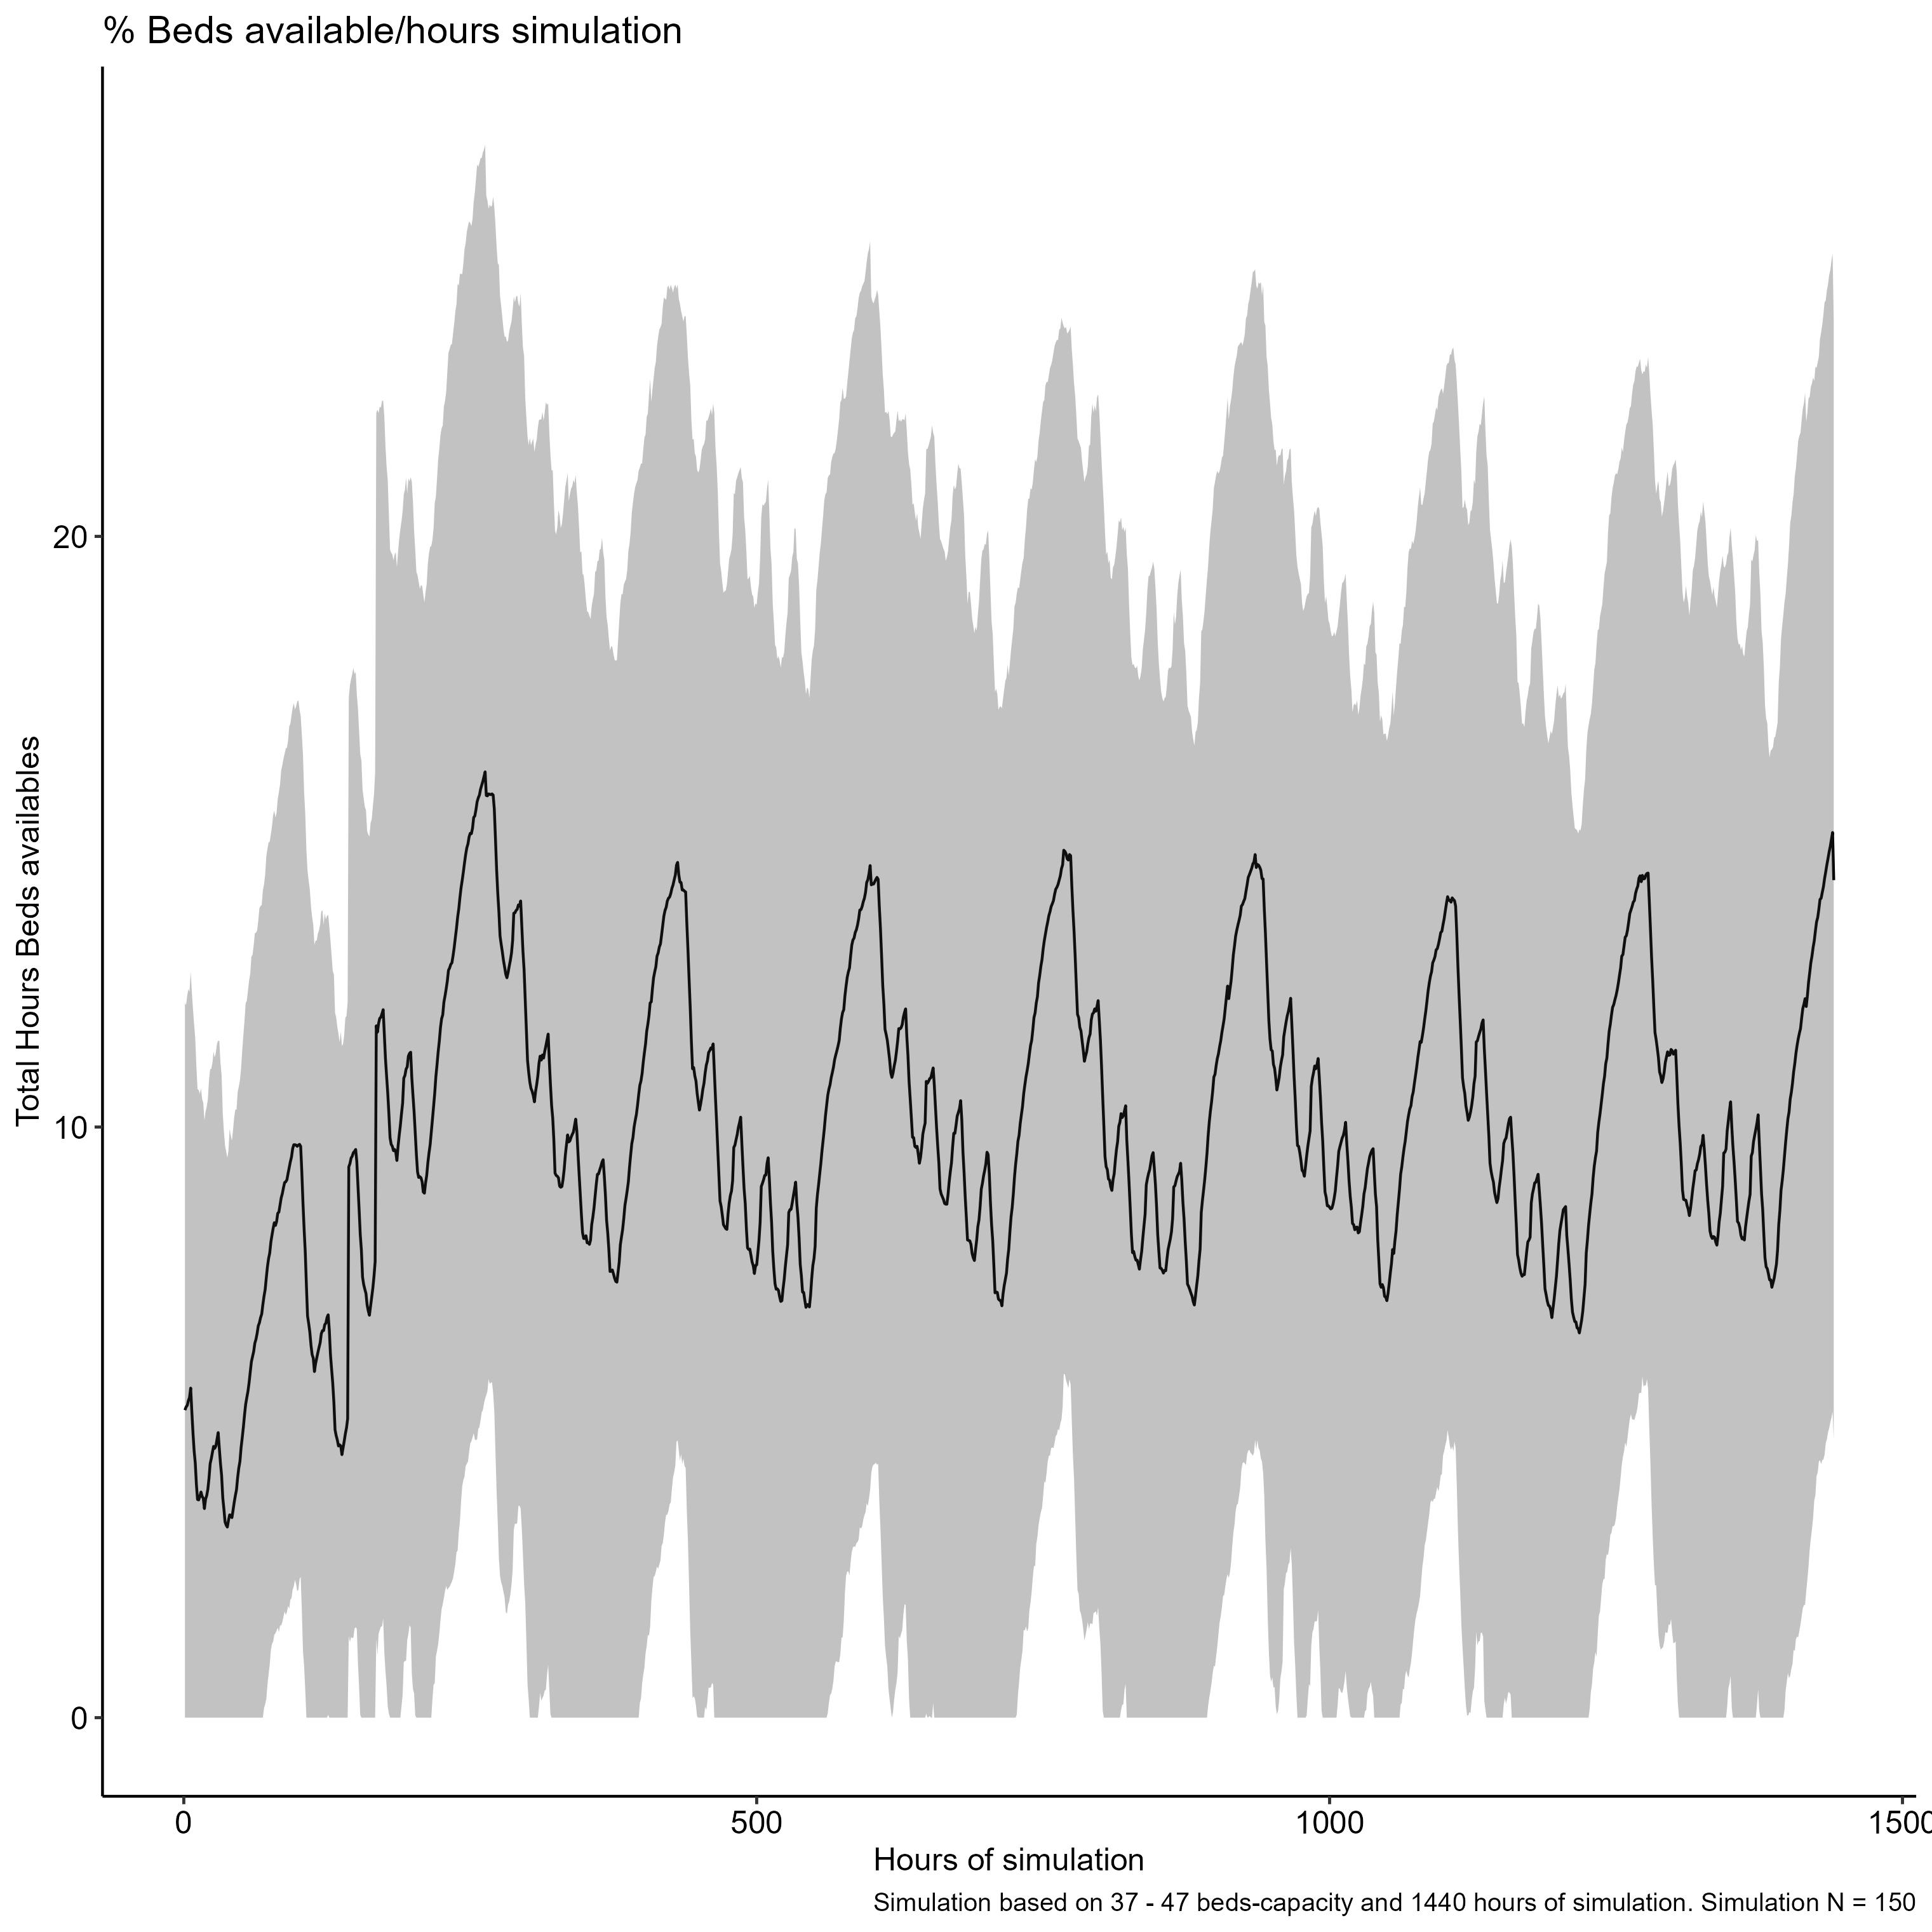
\includegraphics[width=0.8\textwidth]{Image5.jpeg}
\caption{150 simulations of a variable-bed ICU for sixty days with cut-off coefficient of 0.00. It is possible to observe changes in bed occupancy for cyclic difference in admission coefficients.}
\label{fig:coef0.00bedsSimulation}
\end{figure}

%TC:endignore

\end{document}


For 36 fix-beds ICU result show 3030.586 $\pm$ 2113.536 euro/day for regected patients and 14106.49 $\pm$ 601.8003 euro/day for free beds. Totale cost was estimable in euro 17137.08 $\pm$ 2197.544 for day.

    Admission rate for election admission

    L'algoritmo minimizza i costi facendfo accedere prima sui posti letto disponibili  i pazienti in urgenza



### LOS prediction: analysis of the problem and prediction
###Simulation to find best number of beds in fix-beds ICU
###The IntelliICU algorithm to reduce total cost
###Simultion to find a coefficient for IntelliICU algorithm to reduce total cost
